
%(BEGIN_QUESTION)
% Copyright 2015, Tony R. Kuphaldt, released under the Creative Commons Attribution License (v 1.0)
% This means you may do almost anything with this work of mine, so long as you give me proper credit

This wattmeter measures power on one phase of a three-phase power system by sensing both line voltage and line current through instrument transformers.  The nominal line voltage of this power system is 4160 volts AC, while the current may extend upwards of 180 amps AC under full-load conditions:

$$\includegraphics[width=15.5cm]{i01212x01.eps}$$

What would you have to do in order to check the calibration of this wattmeter?  Specifically, devise a step-by-step procedure that you could give to another technician telling them what they would have to do in order to simulate precise amounts of electrical power to the wattmeter's input, keeping safety in mind as the first priority.  Note: you are not allowed to shut power off in the three-phase system to do your test -- it must be done ``live.''

\vskip 10pt

The power of a balanced three-phase system is given by the following formula:

$$P = \sqrt{3} V_{line} I_{line}$$

\vskip 20pt \vbox{\hrule \hbox{\strut \vrule{} {\bf Suggestions for Socratic discussion} \vrule} \hrule}

\begin{itemize}
\item{} An important safety rule to apply when working with live circuit is the ``one-hand rule.''  Explain what this rule is, and how it is applied to a scenario such as this.
\item{} When loosening the screws on a terminal block to remove wires for the PT signal, should you remove the wires from the left-hand side of the terminals (as shown in the diagram) or from the right-hand side, or does this matter at all?  
\item{} The task of disconnecting a wattmeter from live instrument transformers presents significant hazard.  Devise a way to make this procedure safer, using special ``test switches'' installed on the signal wires at the time of construction, so that a technician may simply throw the switches' levers to isolate the wattmeter instead of putting a screwdriver on ``live'' terminals and removing wires from terminal blocks.
\item{} Suppose the PT's output signal were 113.6 volts RMS, and the CT's output signal were 2.9 amps RMS.  How much power does this represent flowing through the three-phase lines?
\item{} Why are both instrument transformers' secondary circuits grounded?
\item{} Suppose the potential transformer has a reliability rating of 0.9995 and the current transformer has a reliability rating of 0.9998.  Calculate the probability that the wattmeter will receive good information from which to calculate power.
\end{itemize}

\underbar{file i01212}
%(END_QUESTION)





%(BEGIN_ANSWER)

The output of a PT is typically somewhere at or below 120 volts AC.  The output of a CT is typically at or below 5 amps AC.  One of the things your procedure must address is how to accurately simulate these voltage and current levels to the wattmeter!

\vskip 10pt

At the given line voltage of 4160 volts the 40:1 ratio PT should output $1 \over 40$ of that (104 volts AC) to the wattmeter's voltage input terminals.  At the maximum line current of 180 amps the 200:5 ratio CT should output $5 \over 200$ of that (4.5 amps AC) to the wattmeter's current input terminals.

%(END_ANSWER)





%(BEGIN_NOTES)

First you must isolate the wattmeter from the signals.  This is done by disconnecting the PT secondary winding from the wattmeter, then short-circuiting the CT secondary winding and then disconnecting that shorted winding from the wattmeter.  Typically, special ``test switches'' are installed for this very purpose, allowing convenient disconnection of PT signals and convenient shorting-then-disconnecting of CT signals.

\vskip 10pt

After disconnecting the wattmeter, the technician would then have to connect a calibration-grade source of AC voltage to the wattmeter's ``V'' terminals, and a calibration-grade source of AC current to the wattmeter's ``I'' terminals.  After injecting known voltage and current quantities, the wattmeter's indication could be checked against the calculated value ($P = \sqrt{3} V_{line} I_{line}$) and any inaccuracies noted.

It should be noted that the voltage and current signals used to test the wattmeter need to be in-phase with each other, otherwise the wattmeter will not register the full amount of power.  True wattmeters account for phase shift between voltage and current (i.e. power factor) in order to register true power ($P$) rather than apparent power ($S$).

\vskip 10pt

At a PT signal of 113.6 VAC and a CT signal of 2.9 AAC, the three-phase (apparent) power will be 912.97 kVA (4.544 kV line voltage at 116 A line current).  If we know that these voltage and current waveforms are in-phase with each other (i.e. power factor = 1) then the true power will also be 912.97 kW.

















\vskip 20pt \vbox{\hrule \hbox{\strut \vrule{} {\bf Virtual Troubleshooting} \vrule} \hrule}

This question is a good candidate for a ``Virtual Troubleshooting'' exercise.  Presenting the diagram to students, you first imagine in your own mind a particular fault in the system.  Then, you present one or more symptoms of that fault (something noticeable by an operator or other user of the system).  Students then propose various diagnostic tests to perform on this system to identify the nature and location of the fault, as though they were technicians trying to troubleshoot the problem.  Your job is to tell them what the result(s) would be for each of the proposed diagnostic tests, documenting those results where all the students can see.

During and after the exercise, it is good to ask students follow-up questions such as:

\begin{itemize}
\item{} What does the result of the last diagnostic test tell you about the fault?
\item{} Suppose the results of the last diagnostic test were different.  What then would that result tell you about the fault?
\item{} Is the last diagnostic test the best one we could do?
\item{} What would be the ideal order of tests, to diagnose the problem in as few steps as possible?
\end{itemize}

%INDEX% Electric power systems: wattmeter connections
%INDEX% Electronics review: current transformer (CT)
%INDEX% Electronics review: potential transformer (PT)

%(END_NOTES)


